\documentclass[11.5pt,a4paper]{article}
\usepackage[utf8x]{inputenc}
\usepackage{graphicx}
\usepackage{subfigure}
\usepackage{color}
\usepackage{xspace}
\usepackage[spanish,es-tabla]{babel} 
%\usepackage[latin1]{inputenc}
\usepackage{amsfonts, amssymb,amsmath}
\usepackage{hyperref} % Required for customizing links
\usepackage{xcolor} % Required for specifying custom colors
\definecolor{dark-blue}{rgb}{0.15,0.15,0.4} % Defines the dark blue color used for links
\hypersetup{colorlinks,linkcolor={dark-blue},citecolor={dark-blue},urlcolor={dark-blue}}
\usepackage{array,booktabs}
\usepackage{multirow, array}
\usepackage{proof}
\usepackage{fancyhdr}
\usepackage{paralist}
\usepackage{marginnote}
\usepackage{float}
\usepackage[top=1.5cm, bottom=1.5cm, outer=1.5cm, inner=1.5cm, heightrounded, marginparwidth=1.5cm, marginparsep=1.5cm]{geometry}
\usepackage{comment}

\begin{document}
\frenchspacing
\begin{center}
    \begin{minipage}{1.9cm}
		\begin{center}
			
\includegraphics[width=1.7cm, height=2.0cm]{logo.png}
		\end{center}
	\end{minipage}
	\begin{minipage}{9.4cm}
		\begin{center}
				{\textsc{Universidad San Francisco de Quito}\\
						  \textsc{\textbf{Curso: Introducción a gnuplot}}\\
						  \textsc{\textbf{Física}} \\
                }
		\end{center}
	\end{minipage}
\end{center}

\thispagestyle{empty}\bigskip
\setlength{\marginparwidth}{5cm}
\small \noindent \textbf{Instructor:}\hspace{0.3cm}Julio César Andrade L.\\
%\small \noindent \textbf{Fecha:}\hspace{0.3cm}\today

\thispagestyle{empty}\bigskip

\par\noindent\rule{\textwidth}{0.4pt}
\vspace{0.5cm}
\begin{center}
\textbf{\large Sobre el curso} 
\end{center}
\vspace{0.5cm}

\small
En este curso aprenderemos a usar las principales herramientas de \texttt{gnuplot} que nos permitiran realizar diferentes tipos de gráficos de datos y funciones de alta calidad (en 2D, 3D) de manera interactiva. 
\vspace{0.5cm}
\normalsize

\section{Sobre gnuplot}

Es una herramienta informática con la utilidad de realizar gráficos de alta calidad a través de la línea de comandos portátil para Linux, OS/2, MS Windows, OSX, VMS y muchas otras plataformas. El código fuente tiene derechos de autor pero se distribuye libremente (es decir, no tiene que pagar por él). Se creó originalmente para permitir que los científicos y los estudiantes visualicen funciones matemáticas y datos de forma interactiva, pero ha crecido para admitir muchos usos no interactivos, como las secuencias de comandos web. También se utiliza como motor de trazado por aplicaciones de terceros como Octave. Gnuplot ha sido apoyado y en desarrollo activo desde 1986.\\* 

Sitio oficial de \texttt{gnuplot}: \url{http://www.gnuplot.info/} 


\section{Instalación}

\begin{itemize}
\item \texttt{En Windows 10:} Lo primero es abrir nuestro navegador de internet e ir a la página oficial de \texttt{gnuplot}: \url{http://www.gnuplot.info/}. Luego hacer click en la pestaña de \texttt{Downloads}, la cual nos rediccionará a la página de \texttt{gnuplot downlads} e inmediatamente debemos hacer click en la prestaña \texttt{Primary download site on SourceForge} que nos rediccionará la vez a otra página donde lo único que tenemos que hacer es darle click al botón derecho de downloads y guardarle como \texttt{.exe}. Una vez ya descargado el archivo \texttt{gnuplot.exe} en el disco duro lo que hacemos es darle doble click y se ejecutará el instalador: luego pedirá seleccionar el idioma con el que vamos a trabajar, después de eso se muestra los términos de licencia del software, de modo que damós en aceptar. Después es solo seguir las intrucciones mostradas (seleccionar la opción de crear enlace en el escritorio) y se instalará de manera rápida el software. Una vez terminado este proceso lo que hacemos es darle doble click en el enlace del programa y ya estamos dentro de \texttt{gnuplot}.    

\item \texttt{En GNU Linux:} Lo primero que debemos abrir es nuestra terminal de comandos y dependiendo de la distribución que tengamos debemos entrar al terminal y ejecutar:

\textit{Debian y sus derivados (ejemplo: Ubuntu)}:\hspace{1.0cm}  \texttt{sudo apt-get install gnuplot}\\
\textit{OPenSuse}:\hspace{5.9cm}  \texttt{sudo zypper install gnuplot}\\
\textit{Fedora, y otros sabores Red Hat}:\hspace{2.6cm}  \texttt{sudo yum install gnuplot}\\
\textit{ArchLinux y derivados}:\hspace{4.0cm}  \texttt{sudo pacman -Syu gnuplot}\\
\textit{Gentoo y derivados}:\hspace{4.5cm} \texttt{sudo emerge -av gnuplot}\\
\textit{Sistemas FreeBSD\/ PcBSD}:\hspace{3.4cm} \texttt{pkg install gnuplot}
\end{itemize}

Realizado lo anterior, lo siguiente es ejecutar el comando \texttt{gnuplot} y automáticamente ya estaremos dentro de \texttt{gnuplot}.

\section{Contenido}

\begin{itemize}
\item \textbf{Primeros Pazos:}\\* 
Familiarización con la línea comandos de gnuplot.\\*
Ploteo de puntos y funciones de una variable.

\item \textbf{Customización de los gráficos:}\\*
Definición de dominio y rango de los gráficos.\\*
Definición tipo, tamaño de los puntos y líneas.\\*
Definición marcas en los ejes.\\*
Definición de título y texto en los ejes de los gráficos.\\*
Definición de posición de la leyenda y customización.\\*
Insertar texto y fórmulas en los gráficos.\\*
Insertar grid en la gráfica.

\item \textbf{Plot gráficos un poco más complejos}\\*
Plot varias curvas en el mismo gráfico y definición del estilo de líneas o puntos de estas curvas.\\*
Plot de \texttt{data}.\\*
Plot gráficos mixtos, data y funciones.\\*
Plot de líneas auxiliares horizontales y verticales.\\*
Cambio a escalar logaritmicas en los ejes.\\*
Exportar gráficos con diferentes formatos (.eps, pdf, png, etc).

\item \textbf{Fitting data}\\*
Interpolación de datos con mínimo cuadrados.\\*
Multiplots.

\item \textbf{Plot de gráficas en 3D}\\*
Gráfico de funciones de dos variables $z = z(x,y)$.\\*
Definción de dominios y rangos de las funciones.\\*
Customización de los ejes del plot.\\*
Plot de \texttt{data} en 3D.\\*
Plot de curvas de nivel.

\item \textbf{Integración con LaTeX}\\*
Inserción de plots (generados en gnuplot) en documentos LaTeX de manera automática.

\end{itemize}

\section{Ejemplos a desarrollar en la clase}

\textbf{Ploteo de puntos}

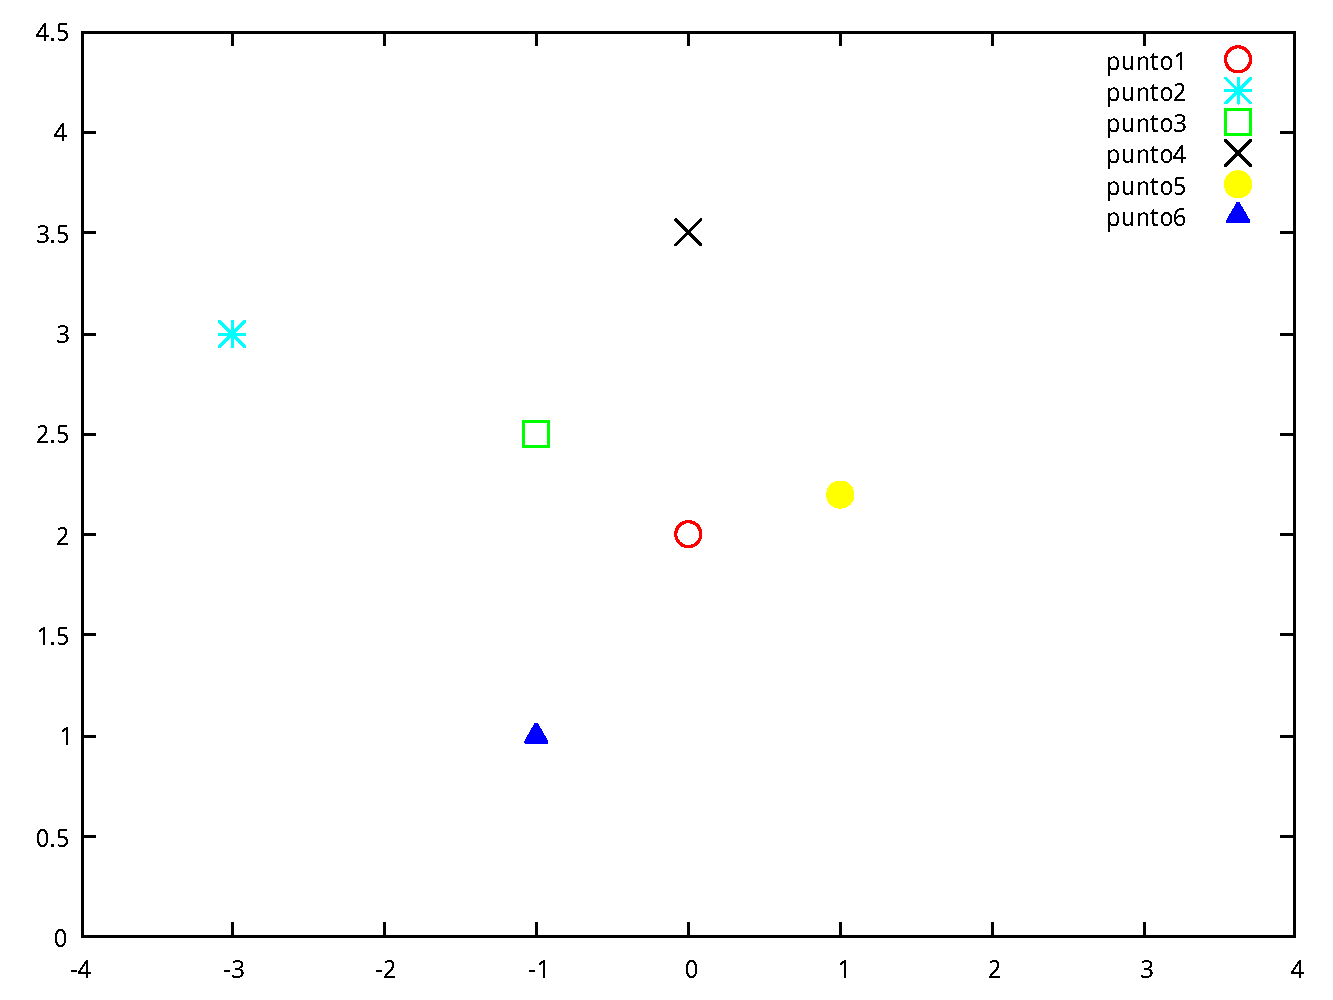
\includegraphics[scale=0.4]{ejemplo1.pdf} 

\textbf{Ploteo de funciones}

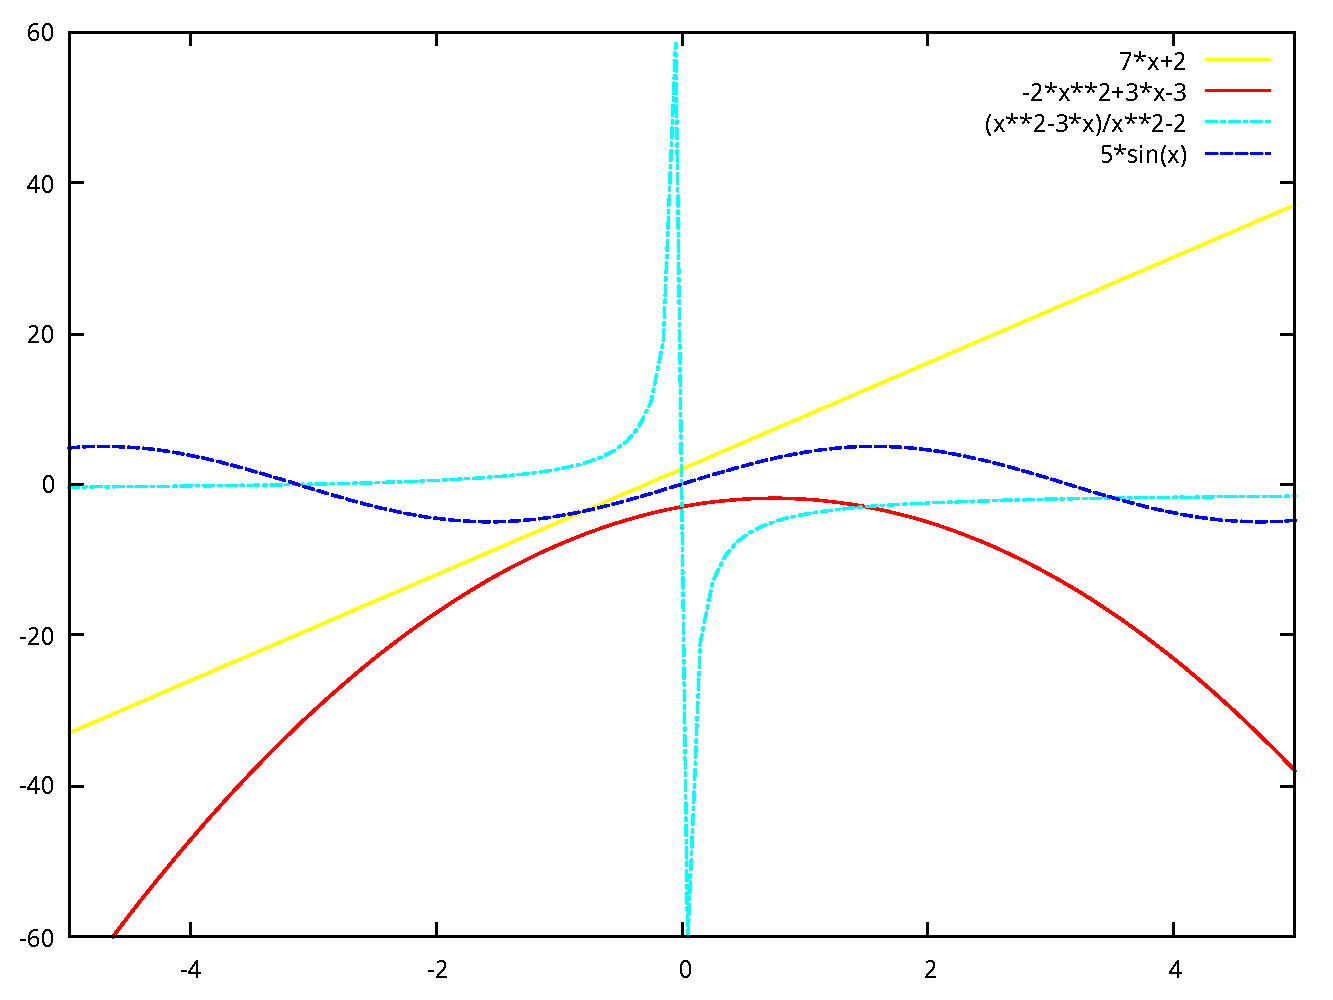
\includegraphics[scale=0.4]{ejemplo2.pdf} 

\textbf{Customización}

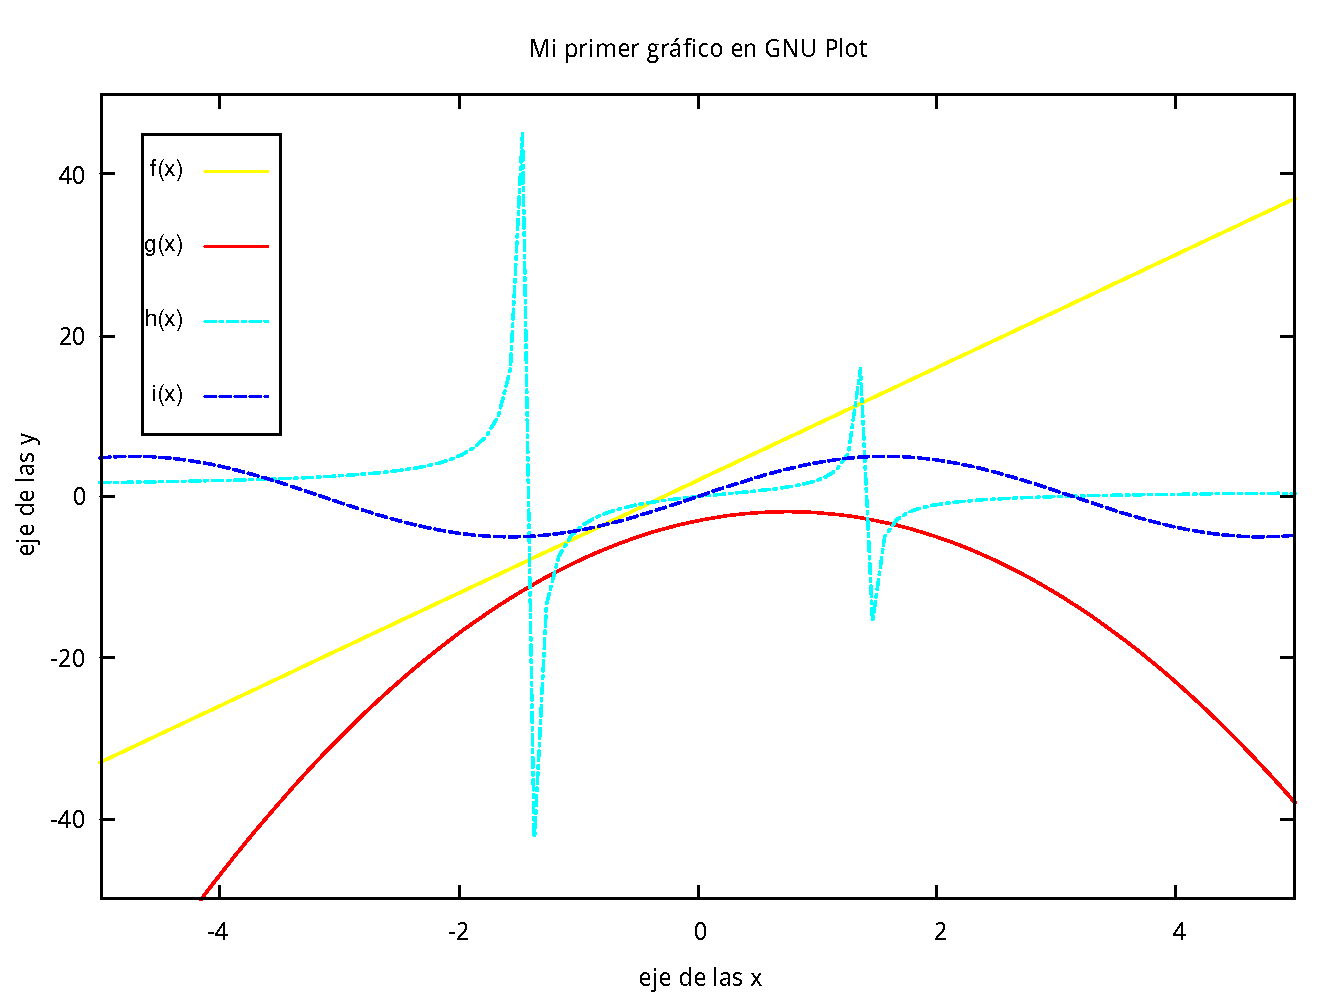
\includegraphics[scale=0.4]{ejemplo3.pdf} 

\textbf{Ejemplo práctico}

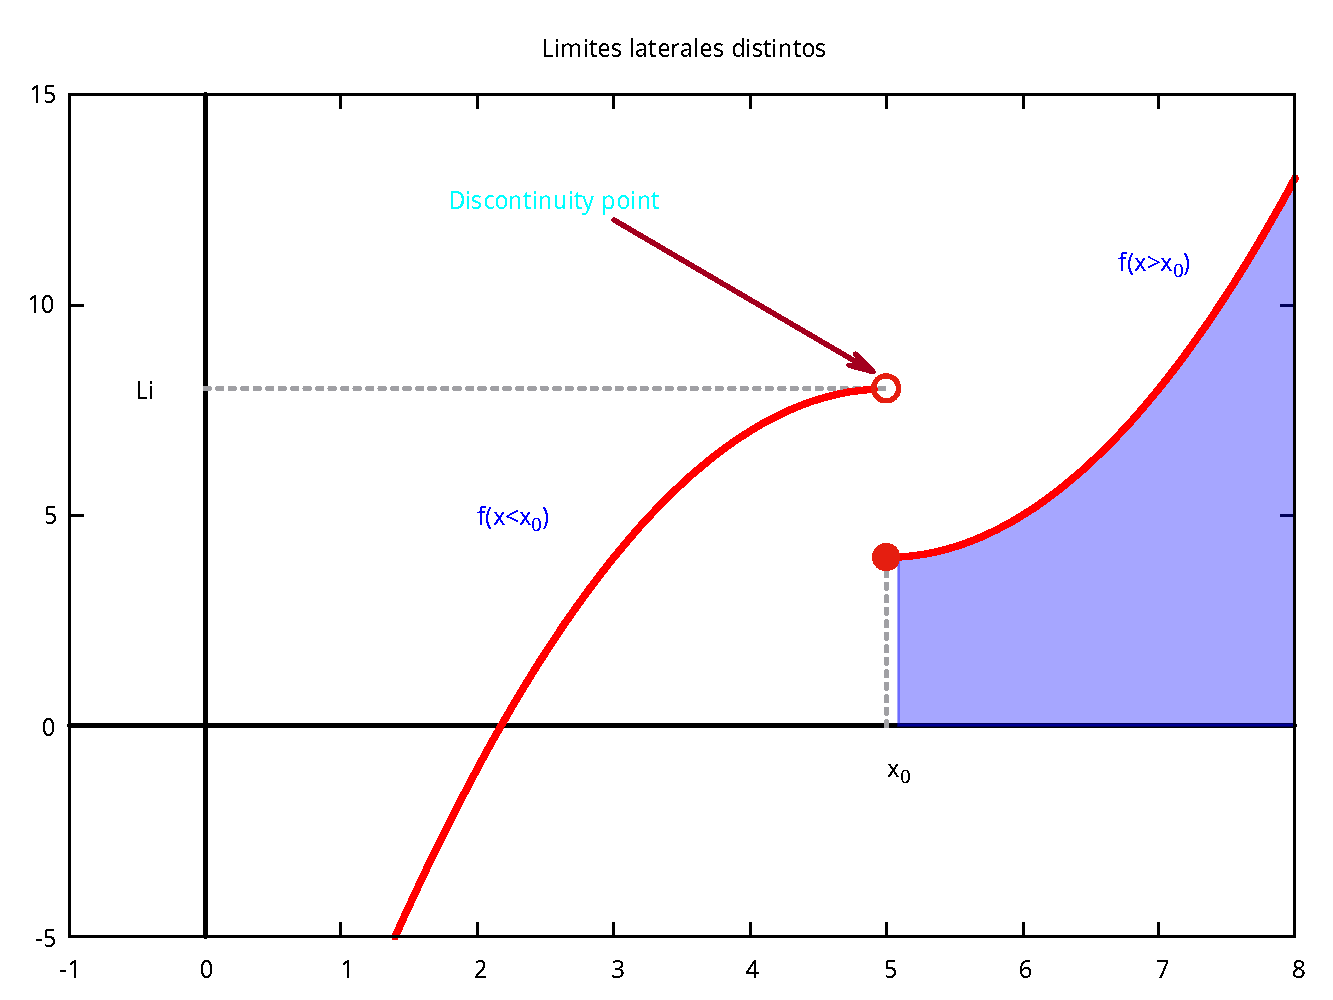
\includegraphics[scale=0.4]{ejemplo4.pdf} 


 

\section{Bibliografía:}

Klein, A., \& Godunov, A., Introductory computational physics. Cambridge University Press, 2006.\\

Rubin H. Landau, Manuel J. Páez, Computational physics: problem solving with Python, 2015.\\

Tao Pang, An introduction to Computational Physics, Cambridge University Press, The
second edition, 2006.


\end{document}
